\documentclass[12pt]{article}
\usepackage{geometry}
\geometry{left=2.25cm, right=2.25cm, top=2.98cm, bottom=2.98cm}
\usepackage{fancyhdr} 
\usepackage{enumerate}
\usepackage{graphicx}
\usepackage{subfigure}
\usepackage{float}
\usepackage{indentfirst}
\usepackage{threeparttable}
\usepackage{hyperref}
\usepackage{diagbox}
\usepackage{tabularx}
\usepackage{bm}
\usepackage{paralist}
\let\itemize\compactitem
\let\enditemize\endcompactitem
\let\enumerate\compactenum
\let\endenumerate\endcompactenum
\let\description\compactdesc
\let\enddescription\endcompactdesc
\hypersetup{
    colorlinks=true,
    linkcolor=blue,
    filecolor=magenta,      
    urlcolor=cyan,
    pdfpagemode=FullScreen,
    }
%Above all for packages
%% Starting here.
\pagestyle{fancy}
\rhead{investigation3}
\addtolength{\topmargin}{-2.49998pt}
\addtolength{\topmargin}{-1.59999pt}
\title{Chemistry Lab Report}
\author{ZHANGYIHENG 10.7 27}
\begin{document}
\maketitle
\begin{center}
    \tableofcontents
\end{center}
\setlength{\parindent}{4ex}
\section{Introduction}
\subsection{Purpose}
The objective of this pratical is to \textbf{determine the concentration of a sodium hydroxide solution (${\rm NaOH}$) } by titrating it against \textbf{a potassium hydrogen phthalate solution }(${\rm KHP}$).\par
\subsection{Background}
A titration measures the volume of solution transported from a buret. In this investigation sodium hydroxide is titrated into a flask with acid . After enough amount of base is added to neutralize the acid in the flask, titration is stopped. The end of titration is indicated by the change of color of phenolphthalein, which is colorless in acidic solution and red-pink in others. \par
Therefore, once the color of the solution turned red-pink, it means the ${\rm NaOH}$ is in excess and the titration is over. We would use the volume of sodium hydroxide solution added to determine the amount of KHP engaged in this reaction and then calculate the concentration of the base.\par
The base is standardized according to the following equation:\par
$${\rm 
KHP \ + \ NaOH \ \to \ KNaP \ + \ H_2O }
$$
\subsection{Apparatuses Used}
\begin{enumerate}
    \item buret
    \item pipette
    \item conical flask
    \item 0.100\textit{M} potassium hydrogen phthalate solution
    \item approximately 0.1\textit{M} sodium hydroxide solution(not exact enough)
    \item phenolphthalein indicator
    \item 3 beakers
    \item iron stand and buret clamp
    \item graduated cylinder
\end{enumerate}
\section{Process of the Experiment}
\subsection{Procedure}
\begin{enumerate}
    \item Obatian 50\textit{ml} of KHP solution in the beaker.
    \item Rinse the pipette and transfer 10.00\textit{ml} of KHP into the conical flask. Then add 15.00\textit{ml} of distilled water and two drops of phenolphthalein into it.
    \item Then do the preparation for titration
    \begin{enumerate}
        \item Rinse burette with distilled water and NaOH solution.
        \item Fill in the base and get rid of the ari bubbles.
        \item Place the conical flask in the right position and adjust the meniscus to origin and record the inital burette reading.
    \end{enumerate}
    \item Titrate the KHP sample and keep shaking the conical flask untill a permanent pink endpoint is reached. Record the reading on the burette wall.
    \item Do the above again and obtain another reading.
\end{enumerate}
\subsection{Data Collected}
\begin{table}[H]
    \centering
    \begin{tabular}{|l|l|l|}
    \hline
        \diagbox{Solution}{Trial}& 1$^{st}$ & 2$^{nd}$ \\ \hline
        Volume (\textit{ml}) & ${\rm 11.23 \pm 0.05}$\ & ${\rm 11.39 \pm 0.05}$ \\ \hline
    \end{tabular}
    \caption{Raw Data Table}
\end{table}
\subsection{Processing Data}
\subsubsection{Volume of NaOH}
First, we need to work out the average value and the uncertainty of the volume, $$\overline{V_{NaOH}} = \frac{11.23 + 11.39}{2} = 11.31ml \ 
\Delta V = 0.05 + 0.05 = 0.10ml$$\par
So we get $$V_{NaOH} = 11.31 \pm 0.10 ml $$
\subsubsection{Concentration of NaOH}
From above we've already obtained that $c_1 = 0.100M$, $V_1 = 10.00ml$, $V_2 = 11.31 \pm 0.10ml$.\par
So we get $$\overline{C_{NaOH}} = \frac{c_1 \times V_1}{\overline{V_2}} \approx 0.088M $$ $$\% \Delta C_{NaOH} = \frac{{\rm Uncertainty}}{{\rm Mean \ Volume}} = \frac{0.10}{11.31} \approx 0.88 \%$$  $$\Delta C_{NaOH} = \pm \overline{C_{NaOH}} \times \% \Delta C_{NaOH} \approx \pm 0.001M$$. 
\subsection{Breif Summary}
During the whole experiment we titrate a sodium hydroxide solution and record volume of it used. After that we use a series of steps to deduce the thickness of the solution to be $(0.088 \pm 0.001)M$.
\section{Conclusion and Evalutaion}
\subsection{Conclusion}
The concentration , as above is $\bm{(0.088 \pm 0.001)}M$, this means one liter of the solution contains $\bm{(0.088 \pm 0.001)}$ moles of solute.\par
Also, molar mass of sodium hydroxide is about $40g/mol$, indicating that solute dissolved in the solution has a mass of $\bm{(0.035 \pm 0.00)g}$ and the thickness can also be represented by $3.095g/l$.
\subsection{Evaluation and Improvements}
\subsubsection{Evaluation}
The concentration of the solution ought be about $0.1M$, but the conclustion we drew above has a percentage dicrepancy of $\displaystyle{\pm \frac{0.088 - 0.100}{0.100}} =\pm 12\%$.\par
However, the concentration we come up with have a relatively small uncertainty of only $ 0.88\%$.As it is much smaller than the percentage one, random error alone cannot account for the discrepancy and hence there must have existed \textbf{some systematic errors} that make our conclusion \textbf{precise but not accurate enough}.\par
\subsubsection{Improvements}
\begin{figure}[H]
    \centering
    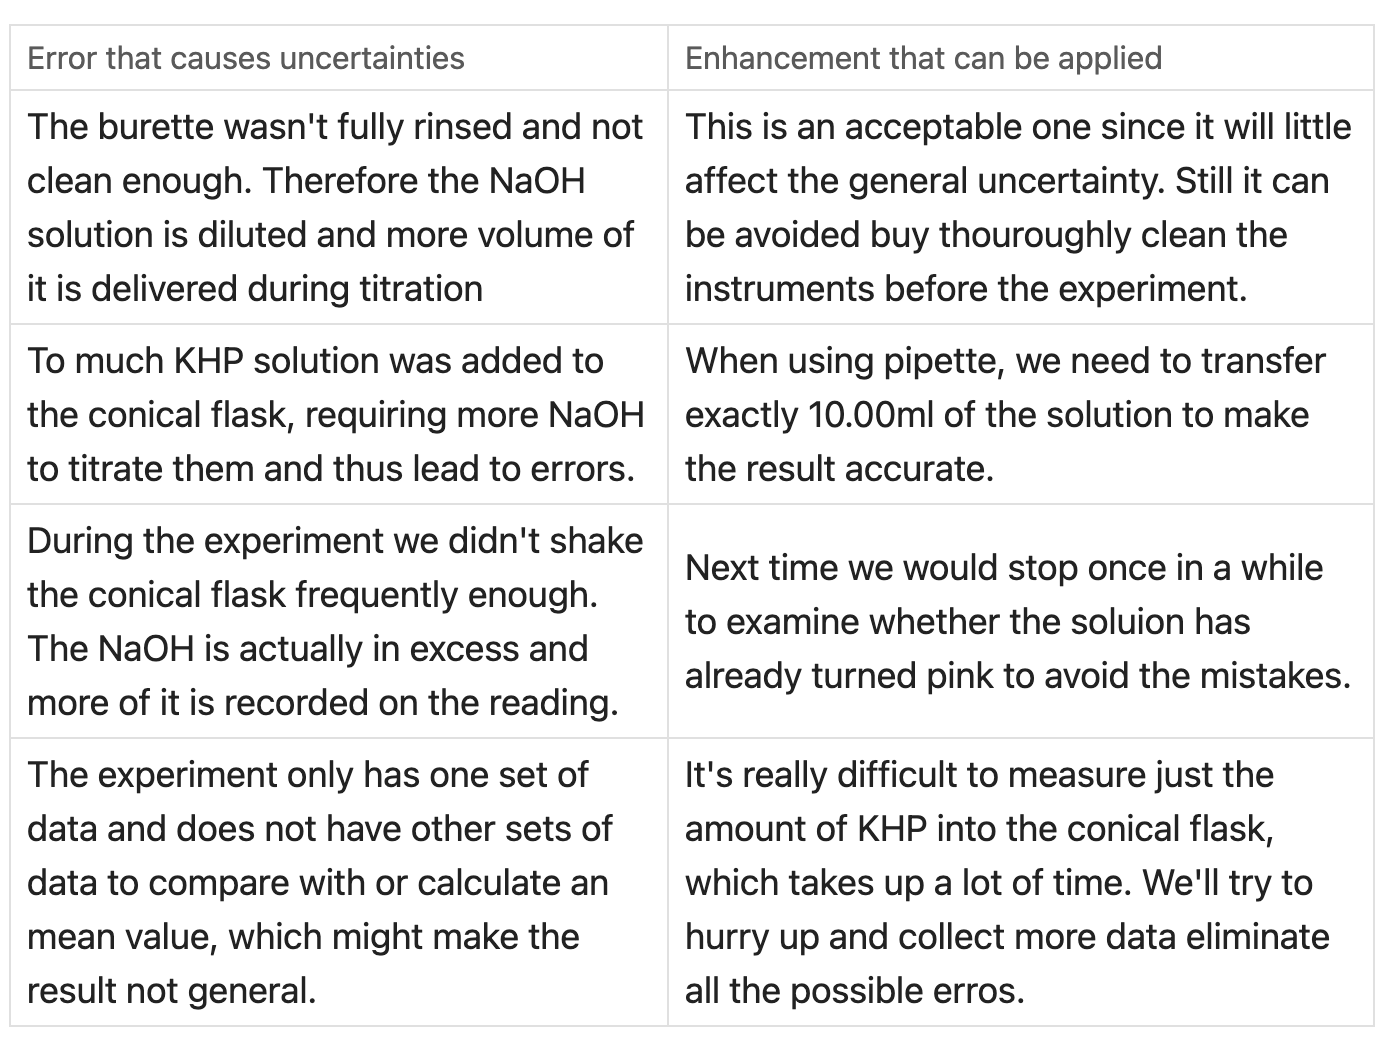
\includegraphics[width = 16cm]{improvments.png}
\end{figure}
\end{document}